%% Nothing to modify here.
%% make sure to include this before anything else

\documentclass[10pt]{beamer}
\usetheme{Szeged}

% packages
\usepackage{color}
\usepackage{listings}

% color definitions
\definecolor{mygreen}{rgb}{0,0.6,0}
\definecolor{mygray}{rgb}{0.5,0.5,0.5}
\definecolor{mymauve}{rgb}{0.58,0,0.82}

% re-format the title frame page
\makeatletter
\def\supertitle#1{\gdef\@supertitle{#1}}%
\setbeamertemplate{title page}
{
  \vbox{}
  \vfill
  \begin{centering}
  \begin{beamercolorbox}[sep=8pt,center]{title}
      \usebeamerfont{supertitle}\@supertitle
   \end{beamercolorbox}
    \begin{beamercolorbox}[sep=8pt,center]{title}
      \usebeamerfont{title}\inserttitle\par%
      \ifx\insertsubtitle\@empty%
      \else%
        \vskip0.25em%
        {\usebeamerfont{subtitle}\usebeamercolor[fg]{subtitle}\insertsubtitle\par}%
      \fi%     
    \end{beamercolorbox}%
    \vskip1em\par
    \begin{beamercolorbox}[sep=8pt,center]{author}
      \usebeamerfont{author}\insertauthor
    \end{beamercolorbox}
    \begin{beamercolorbox}[sep=8pt,center]{institute}
      \usebeamerfont{institute}\insertinstitute
    \end{beamercolorbox}
    \begin{beamercolorbox}[sep=8pt,center]{date}
      \usebeamerfont{date}\insertdate
    \end{beamercolorbox}\vskip0.5em
    {\usebeamercolor[fg]{titlegraphic}\inserttitlegraphic\par}
  \end{centering}
  \vfill
}
\makeatother

% insert frame number
\expandafter\def\expandafter\insertshorttitle\expandafter{%
      \insertshorttitle\hfill%
\insertframenumber\,/\,\inserttotalframenumber}

% preset-listing options
\lstset{
  backgroundcolor=\color{white},   
  % choose the background color; 
  % you must add \usepackage{color} or \usepackage{xcolor}
  basicstyle=\footnotesize,        
  % the size of the fonts that are used for the code
  breakatwhitespace=false,         
  % sets if automatic breaks should only happen at whitespace
  breaklines=true,                 % sets automatic line breaking
  captionpos=b,                    % sets the caption-position to bottom
  commentstyle=\color{mygreen},    % comment style
  % deletekeywords={...},            
  % if you want to delete keywords from the given language
  extendedchars=true,              
  % lets you use non-ASCII characters; 
  % for 8-bits encodings only, does not work with UTF-8
  frame=single,                    % adds a frame around the code
  keepspaces=true,                 
  % keeps spaces in text, 
  % useful for keeping indentation of code 
  % (possibly needs columns=flexible)
  keywordstyle=\color{blue},       % keyword style
  % morekeywords={*,...},            
  % if you want to add more keywords to the set
  numbers=left,                    
  % where to put the line-numbers; possible values are (none, left, right)
  numbersep=5pt,                   
  % how far the line-numbers are from the code
  numberstyle=\tiny\color{mygray}, 
  % the style that is used for the line-numbers
  rulecolor=\color{black},         
  % if not set, the frame-color may be changed on line-breaks 
  % within not-black text (e.g. comments (green here))
  stepnumber=1,                    
  % the step between two line-numbers. 
  % If it's 1, each line will be numbered
  stringstyle=\color{mymauve},     % string literal style
  tabsize=4,                       % sets default tabsize to 4 spaces
  title=\lstname                   
  % show the filename of files included with \lstinputlisting; 
  % also try caption instead of title
}

% macro for code inclusion
\newcommand{\includecode}[2][c]{
	\lstinputlisting[caption=#2, style=custom#1]{#2}
}	% nothing to do here
\usepackage[english]{babel}

\usepackage[utf8]{inputenc}

\newcommand{\course}{
	C introduction
}

\author{
	Richard Mörbitz,
	Manuel Thieme
}

\lstset{
	language = C,
	showspaces = false,
	showtabs = false,
	showstringspaces = false,
	escapechar = @,
	belowskip=-1.5em
} % TODO modify this if you have not already done so

% meta-information
\newcommand{\topic}{
	Pointers
}
\usepackage{tikz}
\usetikzlibrary{arrows}
\tikzset{arrow/.style={-latex, shorten >=.5ex, shorten <=.5ex}}
% nothing to do here
\title{\topic}
\supertitle{\course}
\date{\today}

% the actual document
\begin{document}

\maketitle

\begin{frame}{Contents}
	\tableofcontents
\end{frame}

\section{Overview}
\subsection{}
\begin{frame}{Memory again}
	\begin{tikzpicture}[font=\scriptsize,x=2.5cm]
		
		\draw (0,1) -- (4,1);
		\draw (0,1) -- (0,1.3);
		\draw (0,1.3) -- (4,1.3);
		\draw (4,1) -- (4,1.3);
		
		\node[above=.6em] at (0,1) {\#0};
		\draw[dashed] (.5,1) -- (.5,1.3);
		\node[above=.6em] at (.5,1) {\#4};
		\draw[dashed] (1,1) -- (1,1.3);
		\node[above=.6em] at (1,1) {\#8};
		\draw[dashed] (1.5,1) -- (1.5,1.3);
		\node[above=.6em] at (1.5,1) {\#12};
		\draw[dashed] (2,1) -- (2,1.3);
		\node[above=.6em] at (2,1) {\#16};
		\draw[dashed] (2.5,1) -- (2.5,1.3);
		\node[above=.6em] at (2.5,1) {\#20};
		\draw[dashed] (3,1) -- (3,1.3);
		\node[above=.6em] at (3,1) {\#24};
		\draw[dashed] (3.5,1) -- (3.5,1.3);
		\node[above=.6em] at (3.5,1) {\#28};
		
		\node[blue, below=.4em, right=0em] at (0.15,1.3) {int};
		\draw[dashed, blue] (0,1) -- (.5,1);
		\draw[dashed, blue] (.5,1) -- (.5,1.3);
		\draw[dashed, blue] (0,1.3) -- (.5,1.3);
		\draw[dashed, blue] (0,1) -- (0,1.3);
	
		\node[blue, below=.4em, right=0em] at (.65,1.3) {int};
		\draw[dashed, blue] (.5,1) -- (1,1);
		\draw[dashed, blue] (1,1) -- (1,1.3);
		\draw[dashed, blue] (.5,1.3) -- (1,1.3);
		\draw[dashed, blue] (.5,1) -- (.5,1.3);
		
		\begin{uncoverenv}<2->
			\node[teal, below=.4em, right=0em] at (1.4,1.3) {int*};
			\draw[dashed, teal] (1,1) -- (2,1);
			\draw[dashed, teal] (2,1) -- (2,1.3);
			\draw[dashed, teal] (1,1.3) -- (2,1.3);
			\draw[dashed, teal] (1,1) -- (1,1.3);
		
			\node[teal, below=.4em, right=0em] at (2.4,1.3) {int*};
			\draw[dashed, teal] (2,1) -- (3,1);
			\draw[dashed, teal] (3,1) -- (3,1.3);
			\draw[dashed, teal] (2,1.3) -- (3,1.3);
			\draw[dashed, teal] (2,1) -- (2,1.3);
		
			\node[teal, below=.4em, right=0em] at (3.4,1.3) {int*};
			\draw[dashed, teal] (3,1) -- (4,1);
			\draw[dashed, teal] (4,1) -- (4,1.3);
			\draw[dashed, teal] (3,1.3) -- (4,1.3);
			\draw[dashed, teal] (3,1) -- (3,1.3);
		\end{uncoverenv}		
		
		\begin{uncoverenv}<3->		
			\draw[arrow, teal, bend angle=30, bend left] (1.5,1) to (.75,1);
			\draw[arrow, teal, bend angle=45, bend left] (2.5,1) to (.25,1);
			\draw[arrow, teal, bend angle=70, bend left] (3.5,1) to (.25,1);
		\end{uncoverenv}		
		
		\begin{uncoverenv}<4->
			\draw (.15,.9) -- (.15,.6) node[below]{\textit{int a;}};
			\draw (.75,.9) -- (.75,.6) node[below]{\textit{int b;}};
			\draw (1.5,.9) -- (1.5,.6) node[below]{\textit{int$^*$ pb = \&b;}};
			\draw (2.6,.9) -- (2.6,.6) node[below]{\textit{int$^*$ pa = \&a;}};
			\draw (3.8,.9) -- (3.8,.6) node[below]{\textit{int$^*$ ndpa = \&a;}};
		\end{uncoverenv}
	\end{tikzpicture}
\end{frame}
\begin{frame}{Strings}
	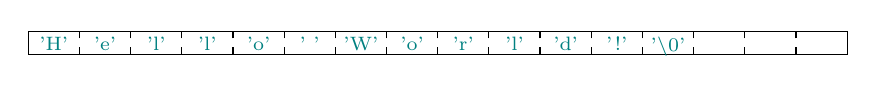
\begin{tikzpicture}[font=\scriptsize,x=1.3cm]
		
		\draw (0,1) -- (8,1);
		\draw (0,1) -- (0,1.3);
		\draw (0,1.3) -- (8,1.3);
		\draw (8,1) -- (8,1.3);
		
		\draw[dashed] (.5,1) -- (.5,1.3);
		\draw[dashed] (1,1) -- (1,1.3);
		\draw[dashed] (1.5,1) -- (1.5,1.3);
		\draw[dashed] (2,1) -- (2,1.3);
		\draw[dashed] (2.5,1) -- (2.5,1.3);
		\draw[dashed] (3,1) -- (3,1.3);
		\draw[dashed] (3.5,1) -- (3.5,1.3);
		\draw[dashed] (4,1) -- (4,1.3);
		\draw[dashed] (4.5,1) -- (4.5,1.3);
		\draw[dashed] (5,1) -- (5,1.3);
		\draw[dashed] (5.5,1) -- (5.5,1.3);
		\draw[dashed] (6,1) -- (6,1.3);
		\draw[dashed] (6.5,1) -- (6.5,1.3);
		\draw[dashed] (7,1) -- (7,1.3);
		\draw[dashed] (7.5,1) -- (7.5,1.3);
		
		\node[teal, below=-.15em] at (.25,1.3) {'H'};
		\node[teal, below=-.15em] at (.75,1.3) {'e'};
		\node[teal, below=-.15em] at (1.25,1.3) {'l'};
		\node[teal, below=-.15em] at (1.75,1.3) {'l'};
		\node[teal, below=-.15em] at (2.25,1.3) {'o'};
		\node[teal, below=-.15em] at (2.75,1.3) {' '};
		\node[teal, below=-.15em] at (3.25,1.3) {'W'};
		\node[teal, below=-.15em] at (3.75,1.3) {'o'};
		\node[teal, below=-.15em] at (4.25,1.3) {'r'};
		\node[teal, below=-.15em] at (4.75,1.3) {'l'};
		\node[teal, below=-.15em] at (5.25,1.3) {'d'};
		\node[teal, below=-.15em] at (5.75,1.3) {'!'};
		\node[teal, below=-.15em] at (6.25,1.3) {'\textbackslash0'};
	\end{tikzpicture}
\end{frame}
% TODO from here on: build your own content


% nothing to do from here on
\end{document}
